\documentclass{standalone}
\usepackage{tikz}
\usetikzlibrary{arrows.meta,bending,positioning,fit}

\begin{document}
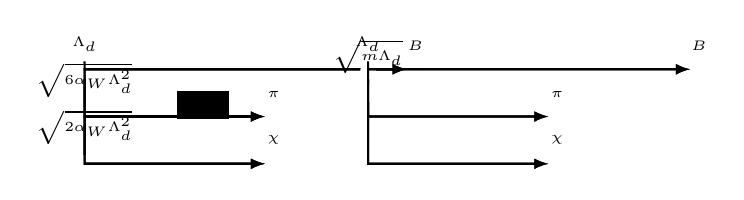
\begin{tikzpicture}[->,>=latex,bend angle=45,font=\tiny,
                    line width=.75pt,scale=.6]
    \node[fill=white,circle,inner sep=2pt,label=above:$B$] (b) at (3,0) {};
    \node[fill=white,circle,inner sep=2pt,label=above:$\pi$]  (pi) at (0,-1) {};
    \node[fill=white,circle,inner sep=2pt,label=above:$\chi$]  (ch) at (0,-2) {};
    \node[fill=white,circle,inner sep=2pt,label=above:$\Lambda_d$,below=2mm] 
     (Ld) at (-4,.5){};
    \node[fill=white,circle,inner sep=2pt,label=above:$\sqrt{6\alpha_W\Lambda_d^2}$] 
     (Ld2) at (-4,-1){};
    \node[fill=white,circle,inner sep=2pt,label=above:$\sqrt{2\alpha_W\Lambda_d^2}$] 
     (Ld3) at (-4,-2){};

    \draw[-{>[scale=1.5]},line width=.75pt] (Ld) -- (Ld |- pi) -- (pi);
    \draw[-{>[scale=1.5]},line width=.75pt] (Ld) -- (Ld |- ch) -- (ch);
    \draw[-{>[scale=1.5]},line width=.75pt] (Ld) -- (Ld |- b) -- (b);
    \draw[-{>[scale=1.5]},line width=.75pt] (Ld2) -- (Ld2 |- pi) -- (pi);
    \draw[-{>[scale=1.5]},line width=.75pt] (Ld2) -- (Ld2 |- ch) -- (ch);
    \draw[-{>[scale=1.5]},line width=.75pt] (Ld2) -- (Ld2 |- b) -- (b);
    \draw[-{>[scale=1.5]},line width=.75pt] (Ld3) -- (Ld3 |- pi) -- (pi);
    \draw[-{>[scale=1.5]},line width=.75pt] (Ld3) -- (Ld3 |- ch) -- (ch);
    \draw[-{>[scale=1.5]},line width=.75pt] (Ld3) -- (Ld3 |- b) -- (b);
    
    \draw[fill=black,ultra thick] (-2,-1)--(-2,-.5)--(-1,-.5)--(-1,-1)--cycle;
    
    \node[fill=white,circle,inner sep=2pt,label=above:$B$] (b2) at (9,0) {};
    \node[fill=white,circle,inner sep=2pt,label=above:$\pi$]  (pi2) at (6,-1) {};
    \node[fill=white,circle,inner sep=2pt,label=above:$\chi$]  (ch2) at (6,-2) {};
    \node[fill=white,circle,inner sep=2pt,label=above:$\Lambda_d$,below=2mm] 
     (Ld2) at (2,.5){};
    \node[fill=white,circle,inner sep=2pt,label=above:$\sqrt{m\Lambda_d}$] 
     (Ld3) at (2,-.5){};
    
    \draw[-{>[scale=1.5]},line width=.75pt] (Ld2) -- (Ld2 |- pi2) -- (pi2);
    \draw[-{>[scale=1.5]},line width=.75pt] (Ld2) -- (Ld2 |- ch2) -- (ch2);
    \draw[-{>[scale=1.5]},line width=.75pt] (Ld2) -- (Ld2 |- b2) -- (b2);
    \draw[-{>[scale=1.5]},line width=.75pt] (Ld3) -- (Ld3 |- pi2) -- (pi2);
    \draw[-{>[scale=1.5]},line width=.75pt] (Ld3) -- (Ld3 |- ch2) -- (ch2);
    \draw[-{>[scale=1.5]},line width=.75pt] (Ld3) -- (Ld3 |- b2) -- (b2);

\end{tikzpicture}
\end{document}